\subsection{Chức năng quản lý tài nguyên (Manage Resources)}
    \begin{figure}[h]
        \centering
        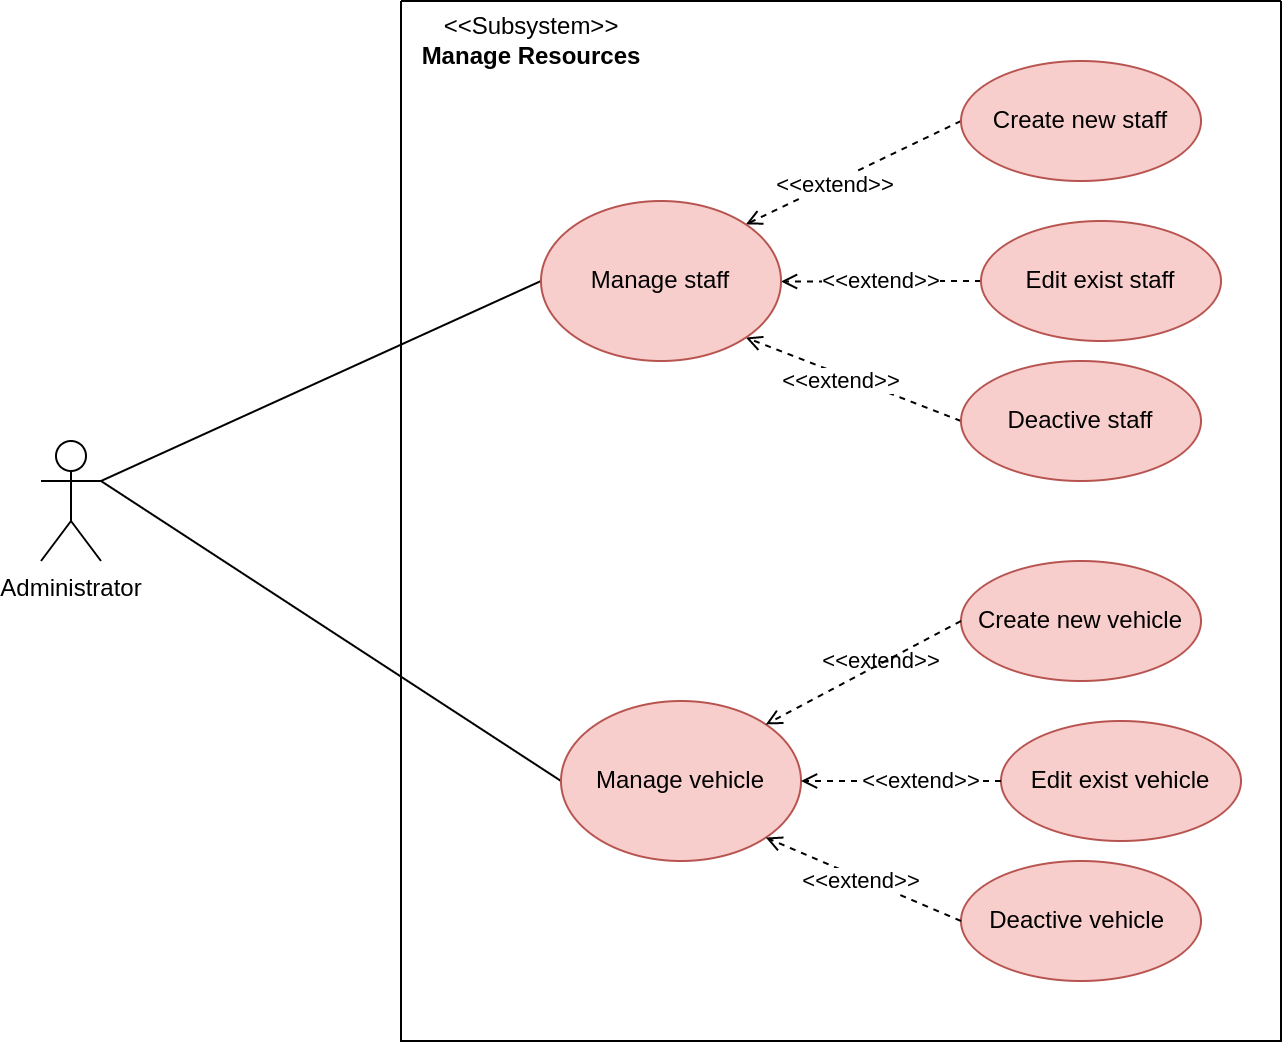
\includegraphics[width=0.70\linewidth]{imgs/use-case diagram/manageResources_uc.png}
        \caption{Use-case diagram chức năng kiểm soát tài nguyên}
    \end{figure}
   
    \vspace{1cm}
    \begin{tblr}{
        width=1\linewidth,
        hlines,
        vlines,
        colspec={X[3]X[7]},
        columns = {valign = m, },
        row{1} = {halign = c, valign = m, bg = lightgray, fg = black},
    }
        {\textbf{Use case name} & \textbf{Manage staff}}  \\
        Description	& Xếp lịch cho nhân viên \\
        Actor & 	Người quản lý (Administrator) \\
        Trigger & 	Người quản lý ấn vào phần quản lý nhân viên \\
        Pre-condition & Người quản lý đang ở quản lý tài nguyên \\
        Post-condition & Trang quản lý nhân viên được hiển thị \\
        Normal flow &   1. Hệ thống lấy dữ liệu về các nhân viên\newline
                    	2. Hệ thống hiện thị danh sách nhân viên lên màn hình \newline
                    	3. Người dùng chọn một nhân viên để thực hiện hành động \newline
                     	4. Hệ thống hiện thị thông tin chi tiết của nhân viên \\
        Extended points & 	Create new staff \newline
                        	Edit exist staff \newline
                        	Deactive staff \\
    \end{tblr}
       
    \begin{tblr}{
        width=1\linewidth,
        hlines,
        vlines,
        colspec={X[3]X[7]},
        columns = {valign = m, },
        row{1} = {halign = c, valign = m, bg = lightgray, fg = black},
    }
        {\textbf{Use case name} & \textbf{Create new staff}}  \\
        Description	& Tạo ra một nhân viên mới \\
        Actor & 	Người quản lý (Administrator) \\
        Trigger & 	Người quản lý ấn vào nút tạo người dùng mới \\
        Pre-condition & Người quản lý đang ở trong phần quản lý nhân viên \\
        Post-condition & Nhân viên mới được tạo ra \\
        Normal flow &   1. Hệ thống hiển thị các thông tin cần điền \newline
                    	2. Người dùng điền các thông tin \newline
                    	3. Hệ thống kiểm tra thông tin được điền \newline
                    	4. Người dùng ấn tạo nhân viên mới \newline
                    	5. Hệ thống ghi nhận nhân viên mới \newline
                    	6. Hệ thống thông báo tạo nhân viên thành công \\
        Alternative flow  & Alternative flow thứ 1: tại bước 1 \newline
                        	1a. Người dùng ấn nút hủy \newline
                        	1b. Quay lại màn hình thông tin chi tiết của nhân viên \\
        Exception flow & Exception flow thứ 1: tại bước 3 \newline
                    	 1a. Nếu thông tin sai, thông báo cho người dùng \newline
                    	 Quay lại bước 2  \\
    \end{tblr}
   
    \vspace{1cm}
    \begin{tblr}{
        width=1\linewidth,
        hlines,
        vlines,
        colspec={X[3]X[7]},
        columns = {valign = m, },
        row{1} = {halign = c, valign = m, bg = lightgray, fg = black},
    }
        {\textbf{Use case name} & \textbf{Edit exist staff}}  \\
        Description	& Chỉnh sửa một nhân viên  \\
        Actor & 	Người quản lý (Administrator) \\
        Trigger & 	Người quản lý ấn vào nút chỉnh sửa nhân viên \\
        Pre-condition & Người quản lý đang ở trong phần quản lý nhân viên \\
        Post-condition & Thông tin nhân viên được chỉnh sửa thành công\\
        Normal flow &   1. Hệ thống hiển thị các thông tin cần điền \newline
                    	2. Người dùng điền các thông tin \newline
                    	3. Hệ thống kiểm tra thông tin được điền \newline
                    	4. Người dùng ấn cập nhật nhân viên \newline
                    	5. Hệ thống ghi nhận thông tin được cập nhật \newline
                    	6. Hệ thống thông báo cập nhật nhân viên thành công \\
        Alternative flow  & Alternative flow thứ 1: tại bước 1 \newline
                        	1a. Người dùng ấn nút hủy \newline
                        	1b. Quay lại màn hình thông tin chi tiết của nhân viên \\
        Exception flow & Exception flow thứ 1: tại bước 3 \newline
                    	 1a. Nếu thông tin sai, thông báo cho người dùng \newline
                    	 Quay lại bước 2 \\
    \end{tblr}
   
    \begin{tblr}{
        width=1\linewidth,
        hlines,
        vlines,
        colspec={X[3]X[7]},
        columns = {valign = m, },
        row{1} = {halign = c, valign = m, bg = lightgray, fg = black},
    }
        {\textbf{Use case name} & \textbf{Deactive staff}}  \\
        Description	& Hủy kích hoạt một nhân viên \\
        Actor & 	Người quản lý (Administrator) \\
        Trigger & 	Người quản lý ấn vào nút hủy kích hoạt nhân viên \\
        Pre-condition & Người quản lý đang ở trong phần quản lý nhân viên \\
        Post-condition & Nhân viên bị hủy kích hoạt\\
        Normal flow &   1. Hệ thống hiểu thị xác nhận hủy kích hoạt nhân viên \newline
                    	2. Người dùng nhấn đồng ý \newline
                    	3. Hệ thống hủy kích hoạt nhân viên \newline
                    	4. Hệ thống thông báo hủy kích hoạt thành công \\
        Alternative flow  & Alternative flow thứ 1: tại bước 1 \newline
                        	1a. Người dùng ấn nút hủy \newline
                        	1b. Quay lại màn hình thông tin chi tiết của nhân viên \\
        Exception flow & none \\
    \end{tblr}
   
    \vspace{1cm}
    \quad Phần use-case senario của  Manage vehicle tương tự như trên.
